% 第 18 题椭圆图：按固定源 PDF 内容流实测值复刻（1 bp → 0.03515 cm）。
% 原点取椭圆中心（源页 (1042.319, 211.881) pdf 坐标），y 向上。
% 椭圆：半长轴 2 cm（56.6936）、半短轴 √2 cm（40.0824），线宽 0.8（源为其余图元 2 倍）；
% 源内三处示意性偏差照源复刻：F 标签处未画真焦点（弦与横轴交点偏内 11.16）、准线取圆整值 2.7 cm（应 2.828 cm，偏内 3.64）、垂直平分线与弦夹角 91.15°（偏 1.15°）。
% 轴：横轴自 −99.21 至箭头尖点 +99.21；纵轴自 −56.69 至 +56.69；箭头为填充三角（3.98×2.99）。
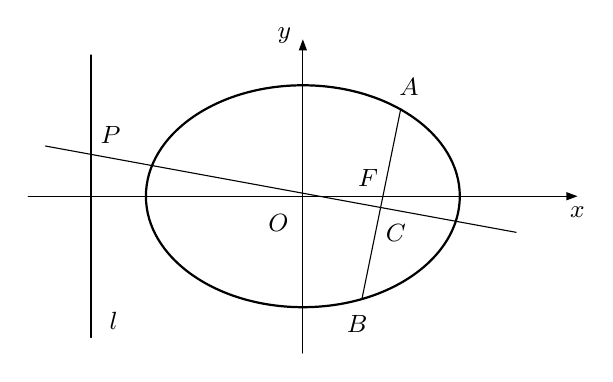
\begin{tikzpicture}[line cap=round,line join=round,font=\small,x=0.03515cm,y=0.03515cm]
% ===== 坐标轴 =====
\draw (-99.21,0)--(95.63,0);   % 横轴（线段止于 1137.95）
\draw (0,-56.69)--(0,53.11);   % 纵轴（线段止于 264.99）
% ===== 轴箭头（填充三角）=====
\fill (99.21,0)--(95.225,1.495)--(95.225,-1.495)--cycle;     % x 轴箭头（顶点 1141.53）
\fill (0,56.69)--(-1.495,52.705)--(1.495,52.705)--cycle;     % y 轴箭头（顶点 268.57）
% ===== 椭圆（中心即原点；a=2 cm、b=√2 cm，源为按 e=√2/2 精确作图）=====
\draw[line width=0.8pt] (0,0) ellipse (56.6936 and 40.0824);
% ===== 准线 l（照源圆整值 2.7 cm）：x = −76.5363，长 ±51.0243 =====
\draw (-76.5363,-51.0243)--(-76.5363,51.0243);
% ===== 弦 AB 与其垂直平分线（照源实测端点）=====
\draw (21.3479,-37.0832)--(35.3937,31.6972);    % 弦 AB（近竖直斜线）
\draw (77.0493,-13.0397)--(-92.9632,18.1363);   % AB 的垂直平分线（贯穿全图，过 C、P）
% ===== 标注（照源字框中心，显式坐标；图内无实心点）=====
\node[anchor=center,inner sep=0] at (-6.649,58.079) {\(y\)};
\node[anchor=center,inner sep=0] at (99.211,-5.596) {\(x\)};
\node[anchor=center,inner sep=0] at (-8.844,-9.681) {\(O\)};
\node[anchor=center,inner sep=0] at (38.301,39.454) {\(A\)};
\node[anchor=center,inner sep=0] at (19.631,-46.281) {\(B\)};
\node[anchor=center,inner sep=0] at (23.526,6.514) {\(F\)};
\node[anchor=center,inner sep=0] at (33.566,-13.341) {\(C\)};
\node[anchor=center,inner sep=0] at (-69.479,22.014) {\(P\)};
\node[anchor=center,inner sep=0] at (-68.364,-44.886) {\(l\)};
\end{tikzpicture}
